\begin{figure}[htbp]
  \centering
  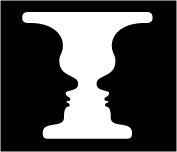
\includegraphics[width=0.35\textwidth]{src/images/vase_of_rubin.png}
  \caption[ルビンの壺]{ルビンの壺：輪郭線の所属先（境界帰属：Border Ownership）を巡り、図（前景）と地（背景）が二峰性にスイッチングする古典的錯視モデル。\newline
  {\footnotesize \textcopyright\ 2007 FeZn, CC BY-SA 3.0 (\url{https://creativecommons.org/licenses/by-sa/3.0/})}}
  \label{fig:rubins_vase}
\end{figure}
